\documentclass[border=10pt]{standalone}
%%%<
\usepackage{verbatim}
%%%>
\begin{comment}
:Title: Highlighting parts of a curves and shading the plane
:Tags: 2D;Functions;Filling;Shading
:Author: lorbj;Elke Schubert
:Slug: highlight-shade

Here we can see how parts of a curve can be emphasized.
A color shading partitions the plane.

The code is from a question by lorbj on TeXwelt.de
http://texwelt.de/wissen/fragen/9875/numerisches-problem-mit-pgfplots
and from the answer by Elke Schubert.

From http://www.pgfplots.net/tikz/examples/highlight-shade/
\end{comment}

\usepackage{pgfplots}
\pgfplotsset{compat=1.10}
\begin{document}
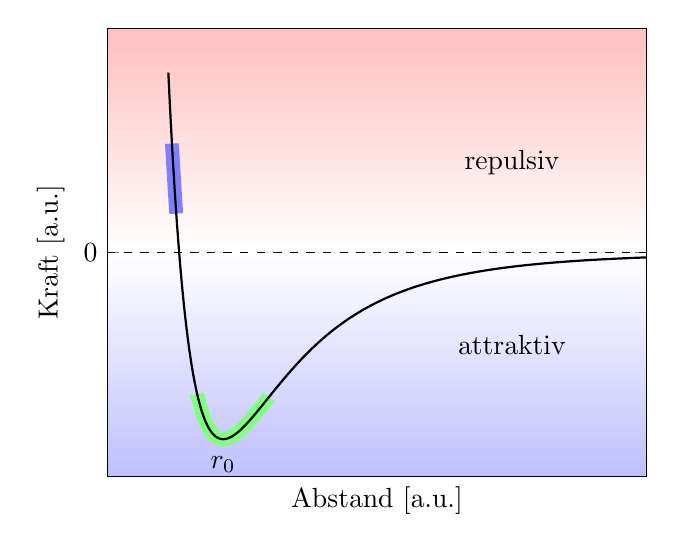
\begin{tikzpicture}
  \begin{axis}[domain  = 0.97:2.3,
               samples = 100,% <- nur 100 statt 400
               xmin    = 0.8,
               xmax    = 2.3,
               ymin    = -0.3,
               ymax    = 0.3,
               ytick   = \empty,
               xtick   = \empty,
               xlabel  = {Abstand [a.u.]},
               ylabel  = {Kraft [a.u.]},
               extra y ticks = {0},
               xlabel near ticks,
               ylabel near ticks,
               set layers,
              ]
    \begin{pgfonlayer}{axis background}
      \fill[shade, top color=blue!0, bottom color=blue!25]
        (rel axis cs:0,0)--(rel axis cs:1,0)--
        (rel axis cs:1,0.5)--(rel axis cs:0,0.5)--cycle;
      \fill[shade, top color=red!25, bottom color=red!0]
        (rel axis cs:0,0.5)--(rel axis cs:1,0.5)--
        (rel axis cs:1,1)--(rel axis cs:0,1)--cycle;
    \end{pgfonlayer}          
    \addplot[line width=5pt,color = green!50, domain = 1.05:1.25]
            {1/x^12-1/x^6};
    \addplot[line width=5pt,color = blue!50,  domain = 0.98:0.992]
            {1/x^12-1/x^6};
    \addplot[thick,
             samples=400% 400 für die Gesamtkurve
            ] {1/x^12-1/x^6};
    \node[anchor= north] at (axis cs: 1.122462048,-0.26) {$r_0$};
    \draw[dashed,thin] (axis cs: 0.8, 0 )-- (axis cs: 2.3, 0);
    \node[anchor = north] at (rel axis cs:0.75,0.75) {repulsiv};
    \node[anchor = south] at (rel axis cs:0.75,0.25) {attraktiv};       
\end{axis}
\end{tikzpicture}
\end{document}
